\documentclass[aspectratio=169,11pt]{beamer}

% ================================================================
% "TABIIY TILNI QAYTA ISHLASH" KURSI
% MA'RUZA 1 --- NLP asoslari va matnni qayta ishlash texnologiyalari
%              (d01_nlp_asoslari.tex)
% Arxetiplar: [A][B][C][D][E] + 4 tsikl [F][G][H][I][J][K][L] +
%             [M][N][O][P][Q][R] + ilova [S]
% Rendered slayd soni: ~41  (L1 uchun ruxsat etilgan istisno: 38-42)
% ================================================================

% ================================================================
% RANGLAR  (asl fayldan o'zgarishsiz)
% ================================================================
\definecolor{cnublue}{rgb}{0.07,0.14,0.62}
\definecolor{cnubluelight}{rgb}{0.18,0.30,0.72}
\definecolor{cnubluebg}{rgb}{0.90,0.92,0.97}
\definecolor{deepblue}{rgb}{0.07,0.14,0.62}
\definecolor{deepred}{rgb}{0.60,0.00,0.00}
\definecolor{deepgreen}{rgb}{0.00,0.45,0.00}
\definecolor{halfgray}{gray}{0.55}

% ================================================================
% BEAMER MAVZU --- Boadilla + maxsus footer  (asl fayldan o'zgarishsiz)
% ================================================================
\usetheme{Boadilla}

\setbeamercolor{structure}{fg=cnublue}
\setbeamercolor{frametitle}{bg=cnublue,fg=white}
\setbeamercolor{title}{bg=cnublue,fg=white}
\setbeamercolor{block title}{bg=cnublue,fg=white}
\setbeamercolor{block body}{bg=cnubluebg,fg=black}
\setbeamercolor{alerted text}{fg=deepred}
\setbeamercolor{author in head/foot}{bg=cnubluelight,fg=white}
\setbeamercolor{section in head/foot}{bg=cnublue,fg=white}
\setbeamercolor{page number in head/foot}{bg=cnubluelight,fg=white}

\setbeamertemplate{mini frame}{}
\setbeamertemplate{mini frame in current section}{}
\setbeamertemplate{mini frame in current subsection}{}
\setbeamertemplate{headline}{}
\setbeamertemplate{navigation symbols}{}

\setbeamertemplate{footline}{%
  \leavevmode%
  \hbox{%
    \begin{beamercolorbox}[wd=0.17\paperwidth,ht=2.5ex,dp=1.25ex,leftskip=0.5em]{author in head/foot}%
      \usebeamerfont{author in head/foot}\scriptsize\insertshortauthor%
    \end{beamercolorbox}%
    \begin{beamercolorbox}[wd=0.69\paperwidth,ht=2.5ex,dp=1.25ex,center]{section in head/foot}%
      \usebeamerfont{section in head/foot}%
      \scriptsize\insertsectionnavigationhorizontal{0.69\paperwidth}{}{}%
    \end{beamercolorbox}%
    \begin{beamercolorbox}[wd=0.14\paperwidth,ht=2.5ex,dp=1.25ex,rightskip=0.5em]{page number in head/foot}%
      \hfill\scriptsize\color{white}%
      \insertframenumber{}/\inserttotalframenumber%
    \end{beamercolorbox}%
  }%
  \vskip0pt%
}

% ================================================================
% PAKETLAR  (asl fayldan o'zgarishsiz)
% ================================================================
\usepackage[utf8]{inputenc}
\usepackage[T1]{fontenc}
\usepackage{lmodern}
\usepackage{amsmath,amssymb}
\usepackage{booktabs}
\usepackage{xcolor}
\usepackage{listings}
\lstset{
    language=Python,
    basicstyle=\ttfamily\scriptsize,
    keywordstyle=\bfseries\color{deepblue},
    emphstyle=\ttfamily\color{deepred},
    stringstyle=\color{deepgreen},
    commentstyle=\itshape\color{halfgray},
    numbers=left,
    numberstyle=\scriptsize\color{halfgray},
    rulesepcolor=\color{cnublue!30},
    frame=shadowbox,
    breaklines=true,
    showstringspaces=false,
    tabsize=2
}
\usepackage{tcolorbox}
\tcbuselibrary{skins}
\tcbset{
  defbox/.style={colback=cnubluebg,colframe=cnublue,
                 fonttitle=\small\bfseries\color{white},
                 attach boxed title to top left={yshift=-2mm,xshift=4mm},
                 boxed title style={colback=cnublue,colframe=cnublue}},
  warnbox/.style={colback=orange!8,colframe=orange!70!black,
                  fonttitle=\small\bfseries},
  okbox/.style={colback=green!7,colframe=green!55!black,
                fonttitle=\small\bfseries}
}
\usepackage{tikz}
\usetikzlibrary{arrows.meta,positioning}

% ================================================================
% QO'SHIMCHALAR  (asl fayldan o'zgarishsiz)
% ================================================================
\AtBeginSection[]{%
  \begin{frame}{Qayerdamiz?}
    \tableofcontents[currentsection]
  \end{frame}}

\newcommand{\bunda}[1]{{\small\textbf{bunda:}\; #1}}
\newcommand{\bajarildi}{{\color{deepgreen}\large$\checkmark$}\;}

% ================================================================
% METAMA'LUMOT
% ================================================================
\title[NLP Asoslari]{NLP Asoslari va Matnni Qayta Ishlash}
\subtitle{Tabiiy tilni qayta ishlash --- 1-ma'ruza}
\author[A.A.\,Abdulali]{A.A.\,Abdulali}
\date{15-iyun 2026}
\institute{11:00--12:20 \quad$\cdot$\quad VMQ 425-son, mavzu \textnumero{}1}

% ================================================================
\begin{document}
% ================================================================

% ----------------------------------------------------------------
% [A] TITUL
% ----------------------------------------------------------------
\maketitle

% ================================================================
\section[Kirish]{Kirish: NLP Nima Uchun?}
% ================================================================

% ----------------------------------------------------------------
% [B] KURS THROUGH-LINE HOOK  (qayta nazorat o'rniga --- birinchi ma'ruza)
% ----------------------------------------------------------------
\begin{frame}{16 Kunda Siz Ishlaydigan NLP Tizimi Qurasiz}
  \begin{columns}[T]
    \begin{column}{0.52\textwidth}
      \textbf{Kapstone loyihasi} --- har dars bir modul:\\[4pt]
      \small
      \begin{itemize}\setlength\itemsep{3pt}
        \item[\textbullet] \textbf{Bugun} (L1 + P1): matn tozalash, BoW, TF-IDF\\
              \texttt{\footnotesize m01\_text\_preprocessor.py}
        \item[\textbullet] \textbf{1-hafta}: klassik tasniflash, vektorlar, qidiruv
        \item[\textbullet] \textbf{2-hafta}: Word2Vec, N-gram, RNN, LSTM
        \item[\textbullet] \textbf{3-hafta}: Transformer, NER, Seq2Seq tarjima
        \item[\textbullet] \textbf{4-hafta}: BERT fine-tuning, RAG, agent, deploy
      \end{itemize}
    \end{column}
    \begin{column}{0.44\textwidth}
      \begin{tcolorbox}[okbox,title=Yakuniy mahsulot]
        \small\textbf{O'zbek Hujjat Yordamchisi}\\[3pt]
        \footnotesize
        Savol $\to$ qidiruv $\to$ kontekst $\to$ javob\\[2pt]
        Sharh $\to$ sentiment tahlil\\[2pt]
        Hujjat $\to$ xulosa chiqarish
      \end{tcolorbox}
      \vspace{4pt}
      \begin{tcolorbox}[warnbox,title=Bugungi ulush]
        \footnotesize
        \texttt{preprocess(text)} funksiyasi ---
        barcha keyingi 14 modul shu funksiyaga
        tayanadi.
      \end{tcolorbox}
    \end{column}
  \end{columns}
\end{frame}

% ----------------------------------------------------------------
% [C] O'QUV MAQSADLARI
% ----------------------------------------------------------------
\begin{frame}{Bugungi Dars Oxirida Siz Nima Qila Olasiz?}
  \begin{enumerate}\setlength\itemsep{8pt}
    \item \textbf{Keltirib chiqara olasiz:}
          NLP ning asosiy vazifalari va ilovalari taksonomiyasini
          (tasniflash, teglash, generatsiya, qidiruv).
    \item \textbf{Amalga oshira olasiz:}
          tokenizatsiya, normalizatsiya, stopword filtrlash, stemming ---
          o'zbek apostrofining Unicode muammosini hisobga olib.
    \item \textbf{Hisoblay olasiz:}
          kichik 3-hujjatli korpus uchun BoW matritsasi va TF-IDF
          qiymatlarini qo'lda.
    \item \textbf{Kodda bog'lay olasiz:}
          \texttt{sklearn.TfidfVectorizer} ni qo'lda hisoblangan
          raqamlar bilan moslashtira olasiz.
  \end{enumerate}
  \vspace{4pt}
  \begin{tcolorbox}[defbox,title=Oldindan talab]
    \footnotesize
    Python asoslari (ro'yxat, tsikl, funksiya);
    maktab darajasida logarifm.
    Eslab qolmagan bo'lsangiz --- ilova slayd \textbf{S1} ga qarang.
  \end{tcolorbox}
\end{frame}

% ----------------------------------------------------------------
% [D] REJA VA VAQT BYUDJETI
% ----------------------------------------------------------------
\begin{frame}{Dars Rejasi: To'rt Tsikl, 80 Daqiqa}
  \begin{center}
  \small
  \begin{tabular}{clcc}
    \toprule
    \textbf{Tsikl} & \textbf{Mavzu} & \textbf{Vaqt} & \textbf{Asosiy chiqish} \\
    \midrule
    1 & NLPga kirish, tarixi, sentiment & 15 daq & Sentiment tahlil tushunchasi \\
    2 & Matnni qayta ishlash (5 bosqich) & 22 daq & Uzbek-aware pipeline + kod \\
    3 & BoW va TF-IDF vektorizatsiya & 25 daq & Qo'lda hisoblangan TF-IDF \\
    4 & NLP vazifalari va ilovalar & 12 daq & Vazifalar xaritasi \\
    \midrule
      & Xulosa, ko'prik P1 ga, savollar & 6 daq & Ertaga nima qurasiz \\
    \bottomrule
  \end{tabular}
  \end{center}
  \vspace{4pt}
  \begin{tcolorbox}[warnbox,title=Har tsikl qanday qurilgan]
    \footnotesize
    intuitsiya $\to$ rasmiy ta'rif $\to$ qo'lda misol $\to$ sizning vazifangiz
    ($\to$ kod ko'prigi). Har qo'lda hisoblangan raqam ertangi P1 da
    \texttt{assert} sifatida tekshiriladi.
  \end{tcolorbox}
\end{frame}

% ----------------------------------------------------------------
% [E] MUAMMO BIRINCHI: NAIVE YONDASHUV XATO BERADI
% ----------------------------------------------------------------
\begin{frame}{Muammo: ``Yaxshi'' Kalit So'zi Salbiy Sharhni Musbat Deb Belgilaydi}
  \begin{columns}[T]
    \begin{column}{0.50\textwidth}
      \textbf{Maqsad}: sharh musbat yoki salbiy?\\[5pt]
      \textbf{Sodda yondashuv}: agar ``yaxshi'' so'zi bo'lsa --- musbat.\\[5pt]
      \begin{tcolorbox}[warnbox,title=Natija xato!,top=2pt,bottom=2pt]
        \small
        \textit{``Bu mahsulot \underline{yaxshi} emas,}\\
        \textit{qaytarib bering!''}\\[3pt]
        naive: ``yaxshi'' topildi\\
        $\Rightarrow$ \textbf{musbat} \hfill\alert{???}
      \end{tcolorbox}
      \vspace{4pt}
      \footnotesize Boshqa muammolar:
      \begin{itemize}\setlength\itemsep{1pt}
        \item So'z tartibi: ``yaxshi emas'' $\ne$ ``emas yaxshi''
        \item Harf katta-kichik: \texttt{YAXSHI} $\ne$ \texttt{yaxshi}
        \item Apostrof: \texttt{o'zbek} $\ne$ \texttt{uzbek}
      \end{itemize}
    \end{column}
    \begin{column}{0.46\textwidth}
      \textbf{NLP yondashuvi:}\\[4pt]
      \begin{enumerate}\small\setlength\itemsep{4pt}
        \item \textbf{Preprocessing} (bugun): tozalash, vektorlash
        \item \textbf{Vektorizatsiya} (bugun): BoW / TF-IDF
        \item \textbf{Model o'qitish}: logistik regressiya (3-ma'ruza)
        \item \textbf{Baholash}: F1, confusion matrix
      \end{enumerate}
      \vspace{5pt}
      \begin{tcolorbox}[okbox,title=Bugun o'rganasiz,top=2pt,bottom=2pt]
        \footnotesize
        1--2 qadamlar: preprocessing va
        vektorizatsiya. Tasniflash ---
        L2 (2-ma'ruza).
      \end{tcolorbox}
    \end{column}
  \end{columns}
\end{frame}

% ================================================================
\section[NLPga kirish]{NLPga Kirish va Tarixi}
% ================================================================

% ----------------------------------------------------------------
% [F1] INTUITSIYA: NLP HAMMA JOYDA
% ----------------------------------------------------------------
\begin{frame}{NLP Hamma Joyda: Siz Ham Undan Foydalanasiz}
  \begin{columns}[T]
    \begin{column}{0.48\textwidth}
      \textbf{Kundalik hayotda NLP:}\\[4pt]
      \small
      \begin{itemize}\setlength\itemsep{4pt}
        \item Spam filtri (Gmail, Outlook)
        \item Matn to'ldirish (Telegram, WhatsApp)
        \item Tarjima (Google Translate)
        \item Ovozli yordamchi (Siri, Alexa)
        \item Qidiruv tizimi (Google, Yandex)
        \item Huquqiy hujjat tahlili (lex.uz)
      \end{itemize}
    \end{column}
    \begin{column}{0.48\textwidth}
      \textbf{Kapstone darsi --- o'zbek NLP:}\\[4pt]
      \small
      \begin{itemize}\setlength\itemsep{4pt}
        \item Uzum Market sharhlar $\to$ sentiment
        \item O'zbek yangiliklari $\to$ tasnif
        \item Hujjatlar bazasi $\to$ semantik qidiruv
        \item So'rov $\to$ RAG asosida javob
      \end{itemize}
      \vspace{6pt}
      \begin{tcolorbox}[defbox,title=Umumiy qonun]
        \footnotesize
        Har qanday matn vazifasi:\\
        \textbf{tozalash $\to$ vektor $\to$ model.}\\
        Bugun --- birinchi ikki qadam.
      \end{tcolorbox}
    \end{column}
  \end{columns}
\end{frame}

% ----------------------------------------------------------------
% [G1] RASMIY TA'RIF + TAKSONOMIYA
% ----------------------------------------------------------------
\begin{frame}{NLP --- Tabiiy Tilni Qayta Ishlash: Rasmiy Ta'rif}
  \begin{tcolorbox}[defbox,title=Ta'rif: NLP (Tabiiy tilni qayta ishlash)]
    \textbf{NLP} (\textit{Natural Language Processing}) ---
    kompyuter fanlari va lingvistikaning kesishmasi;
    maqsad: \textbf{kompyuterlarni inson tili bilan ishlashga o'rgatish}.
  \end{tcolorbox}
  \vspace{5pt}
  \bunda{%
    \textit{corpus} = matnlar to'plami;
    \textit{token} = so'z yoki belgi birligi;
    \textit{label} = tasniflash nishoni
  }
  \vspace{5pt}
  \begin{columns}[T]
    \begin{column}{0.30\textwidth}
      \textbf{Kiritma:}\\[3pt]
      \footnotesize
      Xom matn (string)\\
      Yangiliklar, sharhlar\\
      Huquqiy hujjatlar\\
      Suhbat tarixi
    \end{column}
    \begin{column}{0.36\textwidth}
      \textbf{NLP vazifalari:}\\[3pt]
      \footnotesize
      Tasniflash (classification)\\
      Teglash (tagging / NER)\\
      Generatsiya (generation)\\
      Qidiruv (retrieval)
    \end{column}
    \begin{column}{0.30\textwidth}
      \textbf{Chiqarma:}\\[3pt]
      \footnotesize
      Sinf belgisi\\
      Annotatsiyalangan\\
      ketma-ketlik\\
      Yangi matn
    \end{column}
  \end{columns}
\end{frame}

% ----------------------------------------------------------------
% [H1] TARIX VAQT O'QI
% ----------------------------------------------------------------
\begin{frame}{NLP Tarixi: Qoidalardan Neyron Tarmoqlargacha}
  \begin{center}
  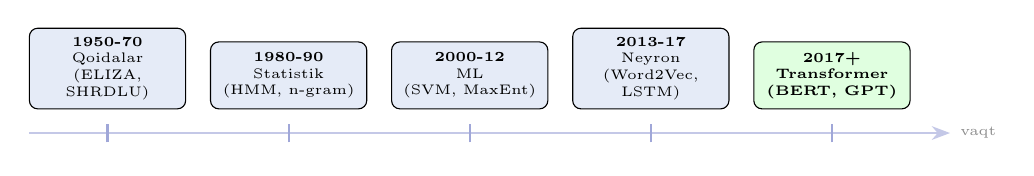
\begin{tikzpicture}[
      era/.style={draw, fill=cnubluebg, rounded corners=3pt,
                  minimum width=1.85cm, minimum height=0.85cm,
                  font=\tiny, text centered, text width=1.75cm},
      gls/.style={draw, fill=green!12, rounded corners=3pt,
                  minimum width=1.85cm, minimum height=0.85cm,
                  font=\tiny\bfseries, text centered, text width=1.75cm}
  ]
    \draw[thick, cnublue!25] (0,0) -- (11.2,0);
    \draw[-{Stealth}, thick, cnublue!25] (11.2,0) -- (11.7,0)
          node[right,font=\tiny,color=halfgray] {vaqt};
    \node[era,   above=3mm] at (1.0,0)  {\textbf{1950-70}\\ Qoidalar\\ (ELIZA, SHRDLU)};
    \node[era,   above=3mm] at (3.3,0)  {\textbf{1980-90}\\ Statistik\\ (HMM, n-gram)};
    \node[era,   above=3mm] at (5.6,0)  {\textbf{2000-12}\\ ML\\ (SVM, MaxEnt)};
    \node[era,   above=3mm] at (7.9,0)  {\textbf{2013-17}\\ Neyron\\ (Word2Vec, LSTM)};
    \node[gls,   above=3mm] at (10.2,0) {\textbf{2017+}\\ Transformer\\ (BERT, GPT)};
    \foreach \x in {1.0,3.3,5.6,7.9,10.2}
      \draw[thick,cnublue!40] (\x,-0.12)--(\x,0.12);
  \end{tikzpicture}
  \end{center}
  \vspace{3pt}
  \begin{columns}[T]
    \begin{column}{0.50\textwidth}
      \textbf{Bu kursda:}\\[3pt]
      \footnotesize
      1-hafta: Statistik + ML (BoW, TF-IDF, LR, NB)\\
      2-hafta: Word2Vec, N-gram, RNN\\
      3-hafta: LSTM, Seq2Seq, Transformer\\
      4-hafta: BERT fine-tuning, RAG, agentlar
    \end{column}
    \begin{column}{0.46\textwidth}
      \begin{tcolorbox}[warnbox,title=O'zbek NLP haqiqati,top=2pt,bottom=2pt]
        \footnotesize
        O'zbek uchun asosiy muammo:
        \textbf{labeled data kamligi}.
        Barcha usullar --- qoidadan
        LLM gacha --- shu muammoni
        turli yo'llar bilan hal qiladi.
      \end{tcolorbox}
    \end{column}
  \end{columns}
\end{frame}

% ----------------------------------------------------------------
% [I1] QO'LDA MISOL: SENTIMENT TAHLIL
% ----------------------------------------------------------------
\begin{frame}{Sentiment Tahlili: Sharh Musbatmi Yoki Salbiy?}
  \textbf{Vazifa}: Uzum Market sharhlarini musbat / salbiy deb tasniflash.
  \vspace{5pt}
  \begin{columns}[T]
    \begin{column}{0.50\textwidth}
      \textbf{Kiritma (xom sharhlar):}\\[5pt]
      \small
      \textit{``Bu dastur juda qulay va tezkor!''}\\[3pt]
      \textit{``Yetkazib berish 3 kun kechikdi.''}\\[3pt]
      \textit{``Narxi yaxshi, lekin sifati o'rtacha.''}
    \end{column}
    \begin{column}{0.46\textwidth}
      \textbf{Maqsad (label):}\\[5pt]
      \small
      $\to$ \textbf{musbat} \textcolor{deepgreen}{\large$+$}\\[3pt]
      $\to$ \textbf{salbiy} \textcolor{deepred}{\large--}\\[3pt]
      $\to$ \textbf{salbiy} \textcolor{deepred}{\large--}
            \quad\footnotesize(``lekin'' zid bildiradi)
    \end{column}
  \end{columns}
  \vspace{7pt}
  \textbf{Sodda pipeline:}
  \begin{enumerate}\small\setlength\itemsep{2pt}
    \item So'zlarni sanash (BoW / TF-IDF) --- \textit{bugun, tsikl 3}
    \item Chastotaga asoslangan model o'qitish (logistik regressiya) --- \textit{L2}
    \item Yangi sharh uchun bashorat
  \end{enumerate}
  \vspace{4pt}
  \textbf{P13 da (14-kun):} BERT ni o'zbek sharhlar uchun fine-tune qilamiz!
\end{frame}

% ----------------------------------------------------------------
% [J1] SIZNING VAZIFANGIZ
% ----------------------------------------------------------------
\begin{frame}{Sizning Vazifangiz: Sentiment Taxmin Qiling}
  \begin{tcolorbox}[warnbox,title=Savol --- 30 soniya]
    \small
    Quyidagi sharh musbatmi yoki salbiy?\\[4pt]
    \textit{``Mahsulot o'z vaqtida keldi, ammo rang kutganimdek emas edi.''}\\[4pt]
    Qaysi so'z yoki ibora sizning qaroringizni belgiladi?
  \end{tcolorbox}
  \pause
  \begin{tcolorbox}[okbox,title=Javob]
    \small
    \textbf{Salbiy} --- ``ammo \ldots{} emas edi'' iborasi salbiy his-tuyg'uni bildiradi.\\[3pt]
    ``O'z vaqtida keldi'' --- musbat signal, lekin ``ammo'' dan keyingisi ustun turadi.\\[3pt]
    \alert{Muammo}: oddiy BoW bu ``ammo''--``emas'' kombinatsiyasini \textbf{ko'rmaydi}
    --- ikkala so'z alohida-alohida hisoblanadi.\\
    Yechim: n-gramlar (5-ma'ruza) yoki BERT (13-ma'ruza).
  \end{tcolorbox}
\end{frame}

% ================================================================
\section[Ishlov berish]{Matnni Qayta Ishlash}
% ================================================================

% ----------------------------------------------------------------
% [F2] INTUITSIYA: XOM MATN SHOVQIN TO'LA
% ----------------------------------------------------------------
\begin{frame}{Xom Matn Shovqin To'la --- Tozalash Shart}
  \begin{columns}[T]
    \begin{column}{0.50\textwidth}
      \textbf{Xom kiritma:}\\[4pt]
      \small\ttfamily
      ``Toshkentda NLP O'RGANISH\\
      JUDA qiziq!!! :) \#nlp''
      \\[7pt]
      \normalfont\small Muammolar:
      \begin{itemize}\footnotesize\setlength\itemsep{2pt}
        \item \texttt{NLP} $\ne$ \texttt{nlp} (harf katta-kichik)
        \item \texttt{!!!}, \texttt{:)}, \texttt{\#nlp} --- shovqin
        \item \texttt{JUDA} --- stopword, ma'no bermaydi
        \item \texttt{O'RGANISH}, \texttt{o'rganish}, \texttt{o'rgan} ---
              bir o'zak, uch alohida token
      \end{itemize}
    \end{column}
    \begin{column}{0.46\textwidth}
      \textbf{Tozalangan chiqarma:}\\[4pt]
      \small\ttfamily
      ['toshkent', 'nlp', 'o'rgan', 'qiziq']
      \\[7pt]
      \normalfont\small Foyda:
      \begin{itemize}\footnotesize\setlength\itemsep{2pt}
        \item Lug'at hajmi kamayadi ($|V|$ $\downarrow$)
        \item Hujjatlar taqqoslanadigan bo'ladi
        \item Bir o'zakli shakllar birga guruhlanadi
      \end{itemize}
      \begin{tcolorbox}[okbox,top=2pt,bottom=2pt]
        \footnotesize
        Preprocessing sifati barcha\\
        keyingi modellar natijasini\\
        bevosita belgilaydi!
      \end{tcolorbox}
    \end{column}
  \end{columns}
\end{frame}

% ----------------------------------------------------------------
% [G2] PREPROCESSING BOSQICHLARI
% ----------------------------------------------------------------
\begin{frame}{Preprocessing Pipeline: Besh Bosqich}
  \begin{tcolorbox}[defbox,title=Ta'rif: Preprocessing pipeline]
    \small
    \begin{enumerate}\setlength\itemsep{3pt}
      \item \textbf{Tokenizatsiya} (\textit{tokenization}) ---
            matnni token ro'yxatiga aylantirish;
            o'zbek uchun Unicode-aware regex zarur
      \item \textbf{Kichik harfga o'tish} (\textit{lowercasing}) ---
            \texttt{NLP}, \texttt{Nlp}, \texttt{nlp} $\to$ \texttt{nlp}
      \item \textbf{Tinish belgilarini tozalash} ---
            \texttt{!}, \texttt{?}, \texttt{:)} $\to$ o'chirish
      \item \textbf{Stop-word filtrlash} (\textit{stopword removal}) ---
            ``va'', ``yoki'', ``bu'', ``ham'' $\to$ o'chirish
      \item \textbf{Stemming} / \textbf{lemmatizatsiya} ---
            ``o'rganadi'' $\to$ ``o'rgan''
    \end{enumerate}
  \end{tcolorbox}
  \vspace{4pt}
  \bunda{%
    \textit{token} = matn birligi;
    \textit{stopword} = ma'nosiz tez-uchraydigan so'z;
    \textit{stem} = so'z o'zagining taxminiy shakli
  }
\end{frame}

% ----------------------------------------------------------------
% [H2a] TOKENIZATSIYA: APOSTROF MUAMMOSI
% ----------------------------------------------------------------
\begin{frame}[fragile]{Tokenizatsiya: O'zbek Apostrofida Yashirin Muammo}
  \begin{columns}[T]
    \begin{column}{0.50\textwidth}
      \textbf{Ingliz uchun oddiy:}\\[3pt]
      \footnotesize\ttfamily
      "it is good".split()\\
      \textrightarrow{} ["it","is","good"]\\[7pt]
      \normalfont\small\textbf{O'zbek uchun murakkab:}\\[3pt]
      \footnotesize
      Apostrofning \textbf{2 turi} mavjud:
      \begin{itemize}\setlength\itemsep{2pt}
        \item ASCII (\texttt{'}) --- klaviatura belgisi (0x27)
        \item Unicode U+2019 (\texttt{'}) --- matn muharrirlari
      \end{itemize}
      \vspace{3pt}
      Byte-darajasida \textbf{TURLI} belgilar!\\[3pt]
      \texttt{nltk.word\_tokenize("o'rganish")}\\
      $\to$ \texttt{["o", "'", "rganish"]}
      \quad\alert{noto'g'ri}
    \end{column}
    \begin{column}{0.46\textwidth}
      \textbf{Yechim --- Unicode-aware regex:}\\[4pt]
      \begin{lstlisting}[numbers=none,frame=single,
                         basicstyle=\ttfamily\tiny]
import re
# ASCII (') va U+2019 (') ikkalasini ushlaydi
pat = re.compile("[a-z\u2019']+")  # '=U+2019

def tokenize_uz(text):
    return pat.findall(text.lower())

# Misol:
tokenize_uz("o'rganish qiziq")
# -> ["o'rganish", "qiziq"]
      \end{lstlisting}
      \begin{tcolorbox}[warnbox,title=P1 eslatma,top=2pt,bottom=2pt]
        \footnotesize
        P1 da ushbu regex
        standart sifatida
        qabul qilinadi.
      \end{tcolorbox}
    \end{column}
  \end{columns}
\end{frame}

% ----------------------------------------------------------------
% [H2b] STOP-WORDS VA STEMMING
% ----------------------------------------------------------------
\begin{frame}{Stop-Words Filtrlash va Stemming: Muhim So'zlarni Qoldiring}
  \begin{columns}[T]
    \begin{column}{0.48\textwidth}
      \textbf{Stop-words (o'zbek misoli):}\\[4pt]
      \small
      \textit{``va'', ``yoki'', ``bu'', ``ham'',\\
      ``lekin'', ``esa'', ``juda'', ``bilan''\ldots}\\[4pt]
      \footnotesize
      Bu so'zlar barcha hujjatlarda tez uchraydi
      $\Rightarrow$ $\mathrm{df}$ yuqori $\Rightarrow$ $\mathrm{IDF}$ past
      $\Rightarrow$ $\mathrm{TF\text{-}IDF}$ past.\\[4pt]
      Filtrlash foydasi: lug'at $|V|$ kamayadi,
      model tezroq va aniqroq.
    \end{column}
    \begin{column}{0.48\textwidth}
      \textbf{Stemming vs Lemmatizatsiya:}\\[3pt]
      \small
      \begin{tabular}{lll}
        \toprule
        So'z & Stem & Lemma \\
        \midrule
        o'rganadi & o'rgan & o'rganmoq \\
        o'rganish & o'rgan & o'rganish \\
        o'rgandim & o'rgan & o'rganmoq \\
        o'rganaman & o'rgan & o'rganmoq \\
        \bottomrule
      \end{tabular}\\[5pt]
      \footnotesize
      \textbf{Stem}: qo'shimcha qirqadi --- tezroq\\
      \textbf{Lemma}: lug'at shakli --- aniqroq\\[3pt]
      O'zbek uchun: Snowball yoki regex.
    \end{column}
  \end{columns}
\end{frame}

% ----------------------------------------------------------------
% [I2] QO'LDA MISOL: BESH BOSQICH
% ----------------------------------------------------------------
\begin{frame}{Qo'lda Misol: Besh Bosqichdan O'tish}
  \textbf{Kiritma:} \texttt{"O'zbekistonda NLP o'rganish juda qiziqarli!"}
  \vspace{5pt}
  \begin{center}
  \begin{tabular}{clp{7.8cm}}
    \toprule
    \textbf{\#} & \textbf{Bosqich} & \textbf{Natija} \\
    \midrule
    1 & Tokenizatsiya &
      \texttt{\tiny["O'zbekistonda","NLP","o'rganish","juda","qiziqarli","!"]} \\[2pt]
    2 & Kichik harf &
      \texttt{\tiny["o'zbekistonda","nlp","o'rganish","juda","qiziqarli","!"]} \\[2pt]
    3 & Tinish tozalash &
      \texttt{\tiny["o'zbekistonda","nlp","o'rganish","juda","qiziqarli"]} \\[2pt]
    4 & Stop-words &
      \texttt{\tiny["o'zbekistonda","nlp","o'rganish","qiziqarli"]}
      \footnotesize\;(\textit{``juda''} olib tashlandi) \\[2pt]
    5 & Stemming &
      \texttt{\tiny["o'zbekiston","nlp","o'rgan","qiziq"]} \\
    \bottomrule
  \end{tabular}
  \end{center}
  \vspace{4pt}
  \begin{tcolorbox}[okbox,title=Muhim kuzatuv,top=2pt,bottom=2pt]
    \footnotesize
    \texttt{"o'rganish"} $\to$ \texttt{"o'rgan"} (stemming).
    Ertaga P1 da barcha 5 bosqich \texttt{TextPreprocessor.preprocess()} metodida
    amalga oshiriladi.
  \end{tcolorbox}
\end{frame}

% ----------------------------------------------------------------
% [J2] SIZNING VAZIFANGIZ: PREPROCESSING
% ----------------------------------------------------------------
\begin{frame}{Sizning Vazifangiz: Matnni Qo'lda Tozalang}
  \begin{tcolorbox}[warnbox,title=Savol --- 2 daqiqa]
    \small
    Quyidagi matnni 5 bosqichdan o'tkazing:\\[4pt]
    \texttt{"Toshkentda katta tadbir bo'ldi, hammaga yoqdi va esda qoldi!"}\\[4pt]
    Stop-words: \{va, yoki, bu, ham, esa, hammaga\}
  \end{tcolorbox}
  \pause
  \begin{tcolorbox}[okbox,title=Javob]
    \footnotesize
    \textbf{1)} \texttt{["Toshkentda","katta","tadbir","bo'ldi","hammaga","yoqdi","va","esda","qoldi","!"]}\\[2pt]
    \textbf{2)} \texttt{["toshkentda","katta","tadbir","bo'ldi","hammaga","yoqdi","va","esda","qoldi","!"]}\\[2pt]
    \textbf{3)} \texttt{["toshkentda","katta","tadbir","bo'ldi","hammaga","yoqdi","va","esda","qoldi"]}\\[2pt]
    \textbf{4)} \texttt{["toshkentda","katta","tadbir","bo'ldi","yoqdi","esda","qoldi"]}\\[2pt]
    \textbf{5)} \texttt{["toshkent","katta","tadbir","bo'l","yoq","esda","qol"]}
  \end{tcolorbox}
\end{frame}

% ----------------------------------------------------------------
% [K2] KOD <-> PIPELINE
% ----------------------------------------------------------------
\begin{frame}[fragile]{Kod $\leftrightarrow$ Pipeline: Uzbek Regex Tokenizer}
  \begin{columns}[T]
    \begin{column}{0.55\textwidth}
\begin{lstlisting}[title=preprocessing\_uz.py]
import re

STOP_UZ = {
    'va', 'yoki', 'bu', 'ham',
    'lekin', 'esa', 'juda'
}

def preprocess(text):
    text = text.lower()          # 2. kichik harf
    tokens = re.findall(         # 1. tokenizatsiya
        "[a-z\u2019']+", text)  # '=U+2019
    tokens = [t for t in tokens  # 4. stopword
              if t not in STOP_UZ]
    stems = [                    # 5. stemming
        re.sub(
          r'(lar|da|dan|ga|ni'
          r'|lik|ish|di|man)$',
          '', t)
        for t in tokens]
    return stems
\end{lstlisting}
    \end{column}
    \begin{column}{0.42\textwidth}
      \textbf{Qator $\to$ bosqich:}\\[4pt]
      \small
      \begin{tabular}{cl}
        \toprule
        Qator & Pipeline bosqich \\
        \midrule
        9  & \#2 kichik harf \\
        10--11 & \#1 tokenizatsiya \\
        12--13 & \#4 stopword filtri \\
        14--19 & \#5 stemming \\
        \bottomrule
      \end{tabular}
      \vspace{5pt}
      \begin{tcolorbox}[warnbox,title=Eslatma,top=2pt,bottom=2pt]
        \footnotesize
        Tinish belgilarini tozalash\\
        (\#3) regex avtomatik:\\
        \texttt{[a-z...]+} faqat\\
        harflarni ushlaydi.
      \end{tcolorbox}
    \end{column}
  \end{columns}
\end{frame}

% ----------------------------------------------------------------
% [L2] TUZOG': APOSTROF BIRLIGI TOKENIZERNI SINDIRADI
% ----------------------------------------------------------------
\begin{frame}{Tuzog': Apostrof Birligi Tokenizer'ni Sindiradi}
  \begin{tcolorbox}[warnbox,title=Haqiqiy xato --- amaliyotda tez-tez uchraydi]
    \small
    Word, Google Docs ko'pincha U+2019 (\texttt{'}) ni ishlatadi.\\[3pt]
    Agar \texttt{re.findall(r"[a-z']+")} da faqat ASCII \texttt{'} (0x27) bo'lsa
    va hujjatda U+2019 (\texttt{'}) bo'lsa:\\[3pt]
    \texttt{"o\textquoteleft{}rganish"} $\to$ \texttt{["o", "rganish"]}
    \quad\alert{NOTO'G'RI}
  \end{tcolorbox}
  \vspace{4pt}
  \begin{tcolorbox}[okbox,title=Yechim: ikkala Unicode nuqtasini qo'llang]
    \small
    \texttt{re.findall(r"[a-z\textbackslash{}u2019']+" , text.lower())}\\[4pt]
    \footnotesize
    \textbackslash{}u2019 = U+2019 (') va \texttt{'} (ASCII 0x27) ikkisini ushlaydi.\\[3pt]
    P1 darsida \texttt{uzbek\_tokenize()} shu regex'ni ishlatadi ---
    bu kurs davomida standart tokenizer sifatida qabul qilinadi.
  \end{tcolorbox}
  \vspace{4pt}
  \footnotesize\color{halfgray}
  Keyingi darsda (L4, 5-kun): Levenshtein masofasi bilan imlo tuzatishda
  ushbu apostrof farqi masofani noto'g'ri hisoblashiga olib keladi.
\end{frame}

% ================================================================
\section[BoW va TF-IDF]{Matn Vektorizatsiyasi}
% ================================================================

% ----------------------------------------------------------------
% [F3] BOW INTUITSIYA
% ----------------------------------------------------------------
\begin{frame}{BoW: Har Bir Hujjat So'zlar To'plami Sifatida}
  \begin{columns}[T]
    \begin{column}{0.40\textwidth}
      \textbf{3 ta hujjat:}\\[6pt]
      \small
      D1: \texttt{"nlp qiziq"}\\[3pt]
      D2: \texttt{"python foydali"}\\[3pt]
      D3: \texttt{"nlp foydali"}\\[10pt]
      \textbf{Lug'at:}\\
      $V = \{\text{nlp, qiziq, python, foydali}\}$
    \end{column}
    \begin{column}{0.56\textwidth}
      \textbf{Har bir so'zni sanash:}\\[4pt]
      \small
      \begin{tabular}{lcccc}
        \toprule
         & nlp & qiziq & python & foydali \\
        \midrule
        D1 & \textbf{1} & \textbf{1} & 0 & 0 \\
        D2 & 0 & 0 & \textbf{1} & \textbf{1} \\
        D3 & \textbf{1} & 0 & 0 & \textbf{1} \\
        \bottomrule
      \end{tabular}\\[6pt]
      \footnotesize
      Har satr --- hujjat vektori $\mathbf{d}_i \in \mathbb{R}^4$.\\
      So'z \textbf{tartibi saqlanmaydi}!\\[3pt]
      \alert{Muammo}: ``nlp'' D1 va D3 da bir xil.\\
      $\to$ Yechim: TF-IDF og'irlash.
    \end{column}
  \end{columns}
\end{frame}

% ----------------------------------------------------------------
% [G3] BOW RASMIY TA'RIF
% ----------------------------------------------------------------
\begin{frame}{So'z Qopi (Bag of Words) --- Rasmiy Ta'rif}
  \begin{tcolorbox}[defbox,title=Ta'rif: So'z qopi (Bag of Words)]
    \textbf{Lug'at}: $V = \{w_1, w_2, \ldots, w_{|V|}\}$ ---
    korpusdagi barcha noyob tokenlar to'plami.\\[5pt]
    \textbf{Hujjat vektori}: $\mathbf{d}_i \in \mathbb{R}^{|V|}$,
    bunda $d_{i,j} = $ ``$w_j$ so'zining $D_i$ hujjatdagi
    paydo bo'lish soni''.
  \end{tcolorbox}
  \vspace{5pt}
  \bunda{%
    $V$ = lug'at; $|V|$ = lug'at hajmi;
    $\mathbf{d}_i$ = $i$-hujjat vektori;
    $d_{i,j}$ = $j$-so'z chastotasi $D_i$ da
  }
  \vspace{5pt}
  \textbf{Muhim xossalar:}\\[3pt]
  \small
  \begin{itemize}\setlength\itemsep{3pt}
    \item $d_{i,j} \geq 0$ \quad (chastota manfiy bo'lmaydi)
    \item $d_{i,j} = 0$ \quad ($w_j$ so'zi $D_i$ da yo'q)
    \item Vektor \textbf{siyrak} (sparse): aksariyat yozuvlar $= 0$
    \item So'z tartibi, kontekst, ma'no --- \alert{yo'qoladi}
  \end{itemize}
\end{frame}

% ----------------------------------------------------------------
% [H3a] TF FORMULA
% ----------------------------------------------------------------
\begin{frame}{TF: Hujjatdagi So'z Chastotasi (Term Frequency)}
  \begin{tcolorbox}[defbox,title=Ta'rif: TF --- atama chastotasi]
    \[
      \mathrm{TF}(t,\, d)
        = \text{(}t\text{ so'zining } d \text{ hujjatdagi paydo bo'lish soni)}
    \]
  \end{tcolorbox}
  \vspace{4pt}
  \bunda{%
    $t$ = so'z (term); $d$ = hujjat (document);
    bu kursda \textbf{raw count} (normalizatsiyasiz) ishlatiadi
  }
  \vspace{5pt}
  \textbf{Misollar (bizning korpus):}
  \begin{center}\small
  \begin{tabular}{llcc}
    \toprule
    Hujjat & Matn & So'z & $\mathrm{TF}$ \\
    \midrule
    D1 & \texttt{"nlp qiziq"} & nlp & $1$ \\
    D1 & \texttt{"nlp qiziq"} & qiziq & $1$ \\
    D2 & \texttt{"python foydali"} & python & $1$ \\
    D3 & \texttt{"nlp foydali"} & foydali & $1$ \\
    \bottomrule
  \end{tabular}
  \end{center}
  \vspace{3pt}
  \footnotesize\color{halfgray}
  Boshqa ta'riflar ham bor (masalan, normalized: $\mathrm{TF}/|d|$).
  Bu kurs raw count ishlatadi --- qo'lda hisoblash osonroq.
\end{frame}

% ----------------------------------------------------------------
% [H3b] IDF FORMULA
% ----------------------------------------------------------------
\begin{frame}{IDF: Noyob So'zlar Mukofotlanadi (Inverse Document Frequency)}
  \begin{tcolorbox}[defbox,title=Ta'rif: IDF --- teskari hujjat chastotasi]
    \[
      \mathrm{IDF}(t)
        = \ln\!\left(\frac{N}{\mathrm{df}(t)}\right)
    \]
  \end{tcolorbox}
  \vspace{4pt}
  \bunda{%
    $N$ = korpusdagi jami hujjatlar soni;
    $\mathrm{df}(t)$ = $t$ uchraydigan hujjatlar soni;
    $\ln$ = natural logarifm
  }
  \vspace{4pt}
  \textbf{Nima uchun logarifm?}
  \begin{itemize}\small\setlength\itemsep{3pt}
    \item Agar $N/\mathrm{df}$ juda katta bo'lsa (noyob so'z),
          $\ln$ shkalani boshqaruvchan qiladi.
    \item $\mathrm{df}(t) = N$: $\mathrm{IDF} = \ln(1) = 0$
          \quad\textcolor{deepred}{(barcha hujjatlarda --- muhim emas)}
    \item $\mathrm{df}(t) = 1$: $\mathrm{IDF} = \ln(N)$
          \quad\textcolor{deepgreen}{(faqat bitta hujjatda --- juda muhim)}
  \end{itemize}
  \vspace{3pt}
  \textbf{TF-IDF}: $\;\mathrm{TF\text{-}IDF}(t, d) = \mathrm{TF}(t,d) \times \mathrm{IDF}(t)$
\end{frame}

% ----------------------------------------------------------------
% [I3] QO'LDA HISOB --- TRACEABILITY SLAYD
%
% P1 (kun-2) birinchi assert bilan solishtiring:
%   TF-IDF('nlp',   D1) = 0.405  [Ma'ruza L1 [I3]-slayd]
%   TF-IDF('qiziq', D1) = 1.099  [Ma'ruza L1 [I3]-slayd]
%
% Korpus: course_map.yaml hand_example verbatim:
%   D1='nlp qiziq', D2='python foydali', D3='nlp foydali'
% ----------------------------------------------------------------
\begin{frame}{Qo'lda Hisob: 3 Hujjat, TF-IDF Matritsasi (P1 Assert Raqamlari)}
  \textbf{Korpus}: $N=3$;\quad
  D1=\texttt{"nlp qiziq"},\; D2=\texttt{"python foydali"},\; D3=\texttt{"nlp foydali"}\\
  $V=\{\text{nlp, qiziq, python, foydali}\}$
  \vspace{4pt}
  \begin{columns}[T]
    \begin{column}{0.44\textwidth}
      \small\textbf{BoW matritsasi:}\\[3pt]
      \begin{tabular}{lcccc}
        \toprule
         & nlp & qiziq & py & foyd \\
        \midrule
        D1 & 1 & 1 & 0 & 0 \\
        D2 & 0 & 0 & 1 & 1 \\
        D3 & 1 & 0 & 0 & 1 \\
        \bottomrule
      \end{tabular}\\[6pt]
      \small\textbf{IDF hisoblash:}\\[3pt]
      \begin{tabular}{lcc}
        \toprule
        So'z & df & IDF \\
        \midrule
        nlp     & 2 & $\ln(3/2)\approx\mathbf{0.405}$ \\
        qiziq   & 1 & $\ln(3/1)\approx\mathbf{1.099}$ \\
        python  & 1 & $\ln(3/1)\approx 1.099$ \\
        foydali & 2 & $\ln(3/2)\approx 0.405$ \\
        \bottomrule
      \end{tabular}
    \end{column}
    \begin{column}{0.52\textwidth}
      \small\textbf{TF-IDF = TF $\times$ IDF:}\\[4pt]
      \begin{align*}
        \mathrm{TF\text{-}IDF}(\text{nlp},\; D1)
          &= 1 \times 0.405 = \mathbf{0.405}\\
        \mathrm{TF\text{-}IDF}(\text{qiziq},\; D1)
          &= 1 \times 1.099 = \mathbf{1.099}
      \end{align*}
      \begin{tcolorbox}[okbox,title=Xulosa,top=2pt,bottom=2pt]
        \footnotesize
        ``qiziq'' D1 ni \textbf{yaxshiroq tavsiflaydi}
        --- faqat D1 da uchraydi! (df=1, IDF yuqori)\\[2pt]
        ``nlp'' D1 ham D3 da bor
        --- past og'irlik ($0.405$).
      \end{tcolorbox}
      \vspace{3pt}
      \footnotesize\color{halfgray}
      Ertangi P1 birinchi assert:\\
      \texttt{abs(val\_nlp - 0.405) < 1e-3}\\
      \texttt{abs(val\_qiziq - 1.099) < 1e-3}\\
      \textit{\# Ma'ruza L1 [I3]-slayd}
    \end{column}
  \end{columns}
\end{frame}

% ----------------------------------------------------------------
% [J3] SIZNING VAZIFANGIZ: TF-IDF(python, D2)
% ----------------------------------------------------------------
\begin{frame}{Sizning Vazifangiz: TF-IDF(\textit{python}, D2) Hisoblang}
  \begin{tcolorbox}[warnbox,title=Savol --- 2 daqiqa (xuddi shu korpus)]
    \small
    D1=\texttt{"nlp qiziq"},\;
    D2=\texttt{"python foydali"},\;
    D3=\texttt{"nlp foydali"},\; $N=3$\\[4pt]
    a) $\mathrm{TF\text{-}IDF}(\text{python},\; D2) = ?$\\[3pt]
    b) $\mathrm{TF\text{-}IDF}(\text{foydali},\; D2) = ?$\\[3pt]
    \footnotesize Qaysi so'z D2 ni yaxshiroq ifodalaydi?
  \end{tcolorbox}
  \pause
  \begin{tcolorbox}[okbox,title=Javob]
    \small
    a)\; $\mathrm{df}(\text{python})=1$
       $\Rightarrow \mathrm{IDF}=\ln(3/1)\approx 1.099$\\
       $\mathrm{TF\text{-}IDF}(\text{python},D2)
         = 1 \times 1.099 = \mathbf{1.099}$\\[4pt]
    b)\; $\mathrm{df}(\text{foydali})=2$\; (D2 va D3 da)
       $\Rightarrow \mathrm{IDF}=\ln(3/2)\approx 0.405$\\
       $\mathrm{TF\text{-}IDF}(\text{foydali},D2)
         = 1 \times 0.405 = \mathbf{0.405}$\\[4pt]
    \textbf{Xulosa:} ``python'' D2 ni yaxshiroq ifodalaydi ---
    faqat D2 da uchraydi!
  \end{tcolorbox}
\end{frame}

% ----------------------------------------------------------------
% [K3] KOD <-> FORMULA BRIDGE
% ----------------------------------------------------------------
\begin{frame}[fragile]{Kod $\leftrightarrow$ Formula: TfidfVectorizer va Qo'lda Hisob}
  \begin{columns}[T]
    \begin{column}{0.54\textwidth}
\begin{lstlisting}[title=tfidf\_demo.py]
from sklearn.feature_extraction.text \
    import TfidfVectorizer

corpus = [
    "nlp qiziq",       # D1
    "python foydali",  # D2
    "nlp foydali"      # D3
]
# smooth_idf=False -> IDF = ln(N/df)
# norm=None -> L2 normalizatsiyasiz
vec = TfidfVectorizer(
    smooth_idf=False, norm=None)
X = vec.fit_transform(corpus).toarray()

idx = vec.vocabulary_
# X[0, idx['nlp']]   -> 0.405
# X[0, idx['qiziq']] -> 1.099
\end{lstlisting}
    \end{column}
    \begin{column}{0.43\textwidth}
      \small\textbf{Parametr $\to$ formula:}\\[4pt]
      \footnotesize
      \begin{tabular}{p{2.7cm}l}
        \toprule
        Parametr & Formula \\
        \midrule
        \texttt{smooth\_idf=False} & $\ln(N/\mathrm{df})$ \\
        \texttt{smooth\_idf=True} & $\ln\frac{N+1}{\mathrm{df}+1}$ \\
        \texttt{norm=None} & raw TF-IDF \\
        \texttt{norm='l2'} & $\ell_2$-norma \\
        \bottomrule
      \end{tabular}
      \vspace{5pt}
      \begin{tcolorbox}[warnbox,title=Ehtiyot,top=2pt,bottom=2pt]
        \footnotesize
        sklearn \textit{default}:\\
        \texttt{smooth\_idf=True},\\
        \texttt{norm='l2'}.\\
        Qo'lda hisob bilan\\
        moslashtirish uchun\\
        parametrlarni\\
        moslang!
      \end{tcolorbox}
    \end{column}
  \end{columns}
\end{frame}

% ================================================================
\section[NLP vazifalari]{NLP Vazifalari va Ilovalari}
% ================================================================

% ----------------------------------------------------------------
% [F4] NLP VAZIFALAR TAKSONOMIYASI
% ----------------------------------------------------------------
\begin{frame}{NLP Nima Qila Oladi? Vazifalar Xaritasi}
  \begin{columns}[T]
    \begin{column}{0.48\textwidth}
      \begin{tcolorbox}[defbox,title=Tasniflash (Classification)]
        \footnotesize
        Matnni sinflarga ajratish\\[2pt]
        \textbullet\; Sentiment: musbat / salbiy\\
        \textbullet\; Spam filtri: spam / ham\\
        \textbullet\; Mavzu: sport, siyosat, \ldots
      \end{tcolorbox}
      \vspace{5pt}
      \begin{tcolorbox}[defbox,title=Teglash (Sequence Labeling)]
        \footnotesize
        Har token uchun sinf belgilash\\[2pt]
        \textbullet\; NER: inson, joy, tashkilot\\
        \textbullet\; POS: ot, fe'l, sifat, \ldots
      \end{tcolorbox}
    \end{column}
    \begin{column}{0.48\textwidth}
      \begin{tcolorbox}[defbox,title=Generatsiya (Generation)]
        \footnotesize
        Yangi matn yaratish\\[2pt]
        \textbullet\; Tarjima: uz $\to$ en\\
        \textbullet\; Xulosa: uzun $\to$ qisqa\\
        \textbullet\; Dialog: savol $\to$ javob
      \end{tcolorbox}
      \vspace{5pt}
      \begin{tcolorbox}[defbox,title=Qidiruv (Retrieval)]
        \footnotesize
        Mos hujjat topish\\[2pt]
        \textbullet\; Semantik qidiruv (FAISS)\\
        \textbullet\; RAG: so'rov $\to$ kontekst $\to$\\
        \quad\quad\quad LLM javob
      \end{tcolorbox}
    \end{column}
  \end{columns}
\end{frame}

% ----------------------------------------------------------------
% [G4] RASMIY VAZIFALAR + O'ZBEK ILOVALAR
% ----------------------------------------------------------------
\begin{frame}{Asosiy NLP Vazifalari va O'zbek Ilovalari}
  \small
  \begin{tabular}{p{2.5cm}p{2.8cm}p{5.5cm}}
    \toprule
    \textbf{Vazifa} & \textbf{Metod} & \textbf{O'zbek ilovasi (kapstone) } \\
    \midrule
    Sentiment tahlil & BoW+LR, BERT & Uzum Market sharhlar (P2, P13) \\
    NER & Bi-LSTM & Lex.uz: shaxs, joy, tashkilot (P10) \\
    Tarjima & Seq2Seq+Attention & Uz-En parallel corpus OPUS-100 (P11) \\
    Xulosa & Transformer & Wikipedia o'zbek maqolalar (P12) \\
    Qidiruv (RAG) & FAISS + LLM & O'zbek qonunchilik hujjatlari (P14) \\
    Agent & LangChain ReAct & Hujjat yordamchisi --- kapstone (P15) \\
    \bottomrule
  \end{tabular}
  \vspace{5pt}
  \begin{tcolorbox}[okbox,title=Kapstone aloqasi,top=2pt,bottom=2pt]
    \footnotesize
    Har satr --- kurs davomida qurasiz. Bugungi preprocessing (m01) barchasining
    birinchi qadami sifatida ishlaydi.
  \end{tcolorbox}
\end{frame}

% ----------------------------------------------------------------
% [I4] TO'LIQ PIPELINE: SHARHDAN SENTIMENT BALLGACHA
% ----------------------------------------------------------------
\begin{frame}{To'liq Pipeline: Sharhdan Sentiment Ballgacha}
  \textbf{Vazifa}: ``Bu mahsulot qimmat, ammo sifati a'lo!'' $\to$ musbat?
  \vspace{6pt}
  \begin{center}
  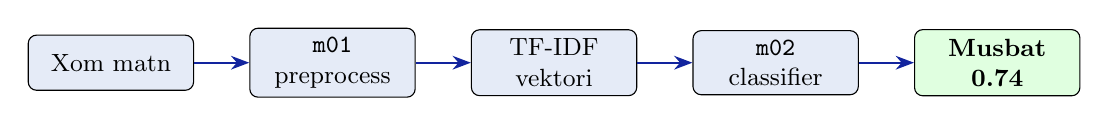
\begin{tikzpicture}[
      box/.style={draw, fill=cnubluebg, rounded corners=3pt,
                  minimum width=2.1cm, minimum height=0.7cm,
                  font=\small, align=center},
      fin/.style={draw, fill=green!12, rounded corners=3pt,
                  minimum width=2.1cm, minimum height=0.7cm,
                  font=\small\bfseries, align=center},
      arr/.style={-{Stealth}, thick, color=cnublue}
  ]
    \node[box] (raw) {Xom matn};
    \node[box, right=0.7cm of raw]  (m01)   {\texttt{m01}\\preprocess};
    \node[box, right=0.7cm of m01]  (tfidf) {TF-IDF\\vektori};
    \node[box, right=0.7cm of tfidf](clf)   {\texttt{m02}\\classifier};
    \node[fin, right=0.7cm of clf]  (out)   {Musbat\\0.74};
    \draw[arr] (raw)--(m01);
    \draw[arr] (m01)--(tfidf);
    \draw[arr] (tfidf)--(clf);
    \draw[arr] (clf)--(out);
  \end{tikzpicture}
  \end{center}
  \vspace{5pt}
  \begin{columns}[T]
    \begin{column}{0.50\textwidth}
      \footnotesize
      \textbf{m01} (bugun):\\
      \texttt{["mahsulot","qimmat","sifat","alo"]}\\[3pt]
      \textbf{TF-IDF}:\\
      $[0.0,\; 0.5,\; 0.3,\; 0.9,\; \ldots]$\\[3pt]
      \textbf{m02} (3-kun): LR bashorat $\to$ \{musbat: 0.74\}
    \end{column}
    \begin{column}{0.46\textwidth}
      \begin{tcolorbox}[warnbox,title=Kuzatuv,top=2pt,bottom=2pt]
        \footnotesize
        ``alo'' so'zining yuqori
        TF-IDF musbat
        tasniflashga yordam beradi.
        ``qimmat'' salbiy signal ---
        model ularni og'irlaydi.
      \end{tcolorbox}
    \end{column}
  \end{columns}
\end{frame}

% ----------------------------------------------------------------
% [J4] SIZNING VAZIFANGIZ: ILOVANI ANIQLANG
% ----------------------------------------------------------------
\begin{frame}{Sizning Vazifangiz: Ilovani NLP Vazifasiga Moslang}
  \begin{tcolorbox}[warnbox,title=Savol --- 2 daqiqa]
    \small
    Quyidagi ilovalar qaysi NLP vazifasiga tegishli?
    \begin{enumerate}\setlength\itemsep{3pt}
      \item Telegram botga ``Bugun Toshkentda ob-havo qanday?'' deb so'rash
      \item Yangiliklar saytida ``NLP'' kalit so'zi bilan mos maqolalar topish
      \item Jurnal maqolasidan 3-gaplik xulosa olish
      \item O'zbek matnida ``Abdulloh Karimov, Toshkent'' ni aniqlash
    \end{enumerate}
  \end{tcolorbox}
  \pause
  \begin{tcolorbox}[okbox,title=Javob]
    \footnotesize
    \begin{enumerate}\setlength\itemsep{2pt}
      \item \textbf{Dialog / Generatsiya} --- LLM agent (P15, 16-kun)
      \item \textbf{Semantik qidiruv / Retrieval} --- FAISS indeks (P14, 15-kun)
      \item \textbf{Xulosa / Summarization} --- Transformer (P12, 13-kun)
      \item \textbf{NER (nomlangan obyektlar)} --- Bi-LSTM (P10, 11-kun)
    \end{enumerate}
  \end{tcolorbox}
\end{frame}

% ================================================================
\section[Xulosa]{Xulosa va Ko'prik}
% ================================================================

% ----------------------------------------------------------------
% [M] O'ZBEK TILI XUSUSIYATLARI (majburiy arxetip)
% ----------------------------------------------------------------
\begin{frame}{O'zbek Tili: Agglutinatsiya TF-IDF Ni Chalg'itadi}
  \begin{columns}[T]
    \begin{column}{0.50\textwidth}
      \textbf{Agglutinativ morfologiya:}\\[4pt]
      \small
      \begin{tabular}{lll}
        \toprule
        Shakl & Morfema tahlili & Stem \\
        \midrule
        o'rganaman & o'rgan+a+man & o'rgan \\
        o'rganish  & o'rgan+ish   & o'rgan \\
        o'rgandim  & o'rgan+di+m  & o'rgan \\
        o'rganadi  & o'rgan+a+di  & o'rgan \\
        \bottomrule
      \end{tabular}\\[5pt]
      \footnotesize
      4 ta \textbf{alohida token} --- 1 ta ma'no!\\
      BoW matritsasida \textbf{4 ta alohida ustun}\\
      (har birida $\mathrm{df}\approx 1$, $\mathrm{IDF}$ yuqori).
    \end{column}
    \begin{column}{0.46\textwidth}
      \textbf{Stemming \textit{olmasa}:}\\[3pt]
      \small
      $\to$ Lug'at hajmi sun'iy oshadi ($|V|\,\uparrow$)\\
      $\to$ Vektor siyraklashadi (sparse $\uparrow$)\\
      $\to$ O'rganish topiklari tarqab ketadi\\[5pt]
      \textbf{Stemming \textit{bilan}:}\\[3pt]
      $\to$ Barcha 4 shakl $\to$ \texttt{"o'rgan"}\\
      $\to$ 1 ta ustun, $\mathrm{df}$ to'g'ri\\[5pt]
      \begin{tcolorbox}[warnbox,title=Dars xulosasi,top=2pt,bottom=2pt]
        \footnotesize
        O'zbek NLP da stemming ---
        \textbf{majburiy}; ingliz tilida
        esa ko'pincha ixtiyoriy.
        m01 uchun asosiy sabablardan biri shu.
      \end{tcolorbox}
    \end{column}
  \end{columns}
\end{frame}

% ----------------------------------------------------------------
% [N] SINTEZ: BOW VS TF-IDF TAQQOSLOV
% ----------------------------------------------------------------
\begin{frame}{Qachon Nima Ishlatish? BoW va TF-IDF Taqqoslov Jadvali}
  \begin{center}\small
  \begin{tabular}{p{2.8cm}p{4.2cm}p{4.2cm}}
    \toprule
    \textbf{Mezon} & \textbf{CountVec (BoW)} & \textbf{TfidfVec} \\
    \midrule
    Asosi & Raw chastota & $\mathrm{TF} \times \mathrm{IDF}$ og'irlash \\
    Umumiy so'zlar & Yuqori $\Rightarrow$ ustunlik & Past $\mathrm{IDF}$ $\Rightarrow$ kamaytiriladi \\
    Noyob so'zlar & Oddiy og'irlik & Yuqori $\mathrm{IDF}$ $\Rightarrow$ muhimroq \\
    Sklearn sinfi & \texttt{CountVectorizer} & \texttt{TfidfVectorizer} \\
    Tezlik & Tezroq & Ozgina sekinroq \\
    Qo'llash & Baseline, Naive Bayes & Qidiruv, LR, SVM \\
    O'zbek uchun & Stemming kerak & Stemming + IDF muhim \\
    \bottomrule
  \end{tabular}
  \end{center}
  \vspace{4pt}
  \begin{tcolorbox}[okbox,title=Amaliy qoida,top=2pt,bottom=2pt]
    \footnotesize
    Har doim \texttt{TfidfVectorizer} bilan boshlang;
    Naive Bayes uchun \texttt{CountVectorizer} ni sinab ko'ring.
    Ikkalasida ham preprocessor (m01) majburiy.
  \end{tcolorbox}
\end{frame}

% ----------------------------------------------------------------
% [O] SEMINAL MANBA + MUHOKAMA SAVOLI
% ----------------------------------------------------------------
\begin{frame}{Salton (1975): 50 Yillik Poydevor}
  \begin{tcolorbox}[defbox,title=Seminal maqola]
    \small
    Salton, G., Wong, A., Yang, C.S.\ (1975).
    \textbf{A Vector Space Model for Automatic Indexing.}
    \textit{Communications of the ACM}, 18(11), 613--620.
  \end{tcolorbox}
  \vspace{5pt}
  \textbf{Maqola haqida:}
  \begin{itemize}\small\setlength\itemsep{3pt}
    \item 1975 --- Google'dan 23 yil oldin!
    \item Matnni vektor sifatida ko'rish g'oyasi shu erdan boshlanadi
    \item TF-IDF og'irlash shu maqoladan kelib chiqqan
    \item Bugungi BERT, GPT ham ``embedding'' g'oyasiga tayanadi
    \item Google Scholar: 10 000+ iqtibos
  \end{itemize}
  \vspace{5pt}
  \begin{tcolorbox}[warnbox,title=Keyingi sessiyaga muhokama savoli]
    \small
    TF-IDF ``qiziq'' ni D1 uchun muhim so'z deb aniqladi.\\
    Ammo \textbf{``qiziq'' va ``qiziqarli''} ni bir xil ma'no deb ko'ra oladimi?\\
    Nima yetishtirmayapti? (P1 da muhokama qilamiz.)
  \end{tcolorbox}
\end{frame}

% ----------------------------------------------------------------
% [P] MAQSADLAR BAJARILDI
% ----------------------------------------------------------------
\begin{frame}{Bugungi Maqsadlar Bajarildi}
  \begin{enumerate}\setlength\itemsep{10pt}
    \item \bajarildi \textbf{Keltirib chiqardik:}
          NLP vazifalari taksonomiyasi --- tasniflash, teglash,
          generatsiya, qidiruv; O'zbek kapstone ilovalari.
    \item \bajarildi \textbf{Amalga oshirdik:}
          tokenizatsiya, normalizatsiya, stopword filtrlash, stemming ---
          o'zbek apostrofining U+2019 muammosi bilan birga.
    \item \bajarildi \textbf{Hisobladik:}
          3 hujjatli korpus uchun BoW matritsasi;
          $\mathrm{IDF(nlp)}\approx 0.405$,
          $\mathrm{TF\text{-}IDF(qiziq,D1)}\approx 1.099$.
    \item \bajarildi \textbf{Kodda bog'ladik:}
          \texttt{TfidfVectorizer(smooth\_idf=False, norm=None)} ni
          qo'lda hisoblangan qiymatlar bilan moslashtirdik.
  \end{enumerate}
\end{frame}

% ----------------------------------------------------------------
% [Q] KO'PRIK: ERTAGA P1
% ----------------------------------------------------------------
\begin{frame}{Ertaga P1: Preprocessing Pipeline Qurasiz}
  \begin{center}
  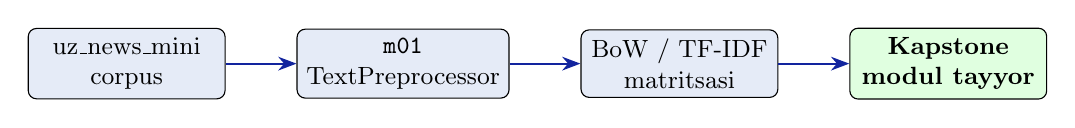
\begin{tikzpicture}[
      mod/.style={draw, fill=cnubluebg, rounded corners=3pt,
                  minimum width=2.5cm, minimum height=0.75cm,
                  font=\small, align=center},
      fin/.style={draw, fill=green!12, rounded corners=3pt,
                  minimum width=2.5cm, minimum height=0.75cm,
                  font=\small\bfseries, align=center},
      arr/.style={-{Stealth}, thick, color=cnublue}
  ]
    \node[mod] (raw) {uz\_news\_mini\\corpus};
    \node[mod, right=0.9cm of raw] (m01) {\texttt{m01}\\TextPreprocessor};
    \node[mod, right=0.9cm of m01] (vec) {BoW / TF-IDF\\matritsasi};
    \node[fin, right=0.9cm of vec] (cap) {Kapstone\\modul tayyor};
    \draw[arr] (raw)--(m01);
    \draw[arr] (m01)--(vec);
    \draw[arr] (vec)--(cap);
  \end{tikzpicture}
  \end{center}
  \vspace{6pt}
  \begin{columns}[T]
    \begin{column}{0.50\textwidth}
      \textbf{P1 da qurasiz:}\\[3pt]
      \small
      \begin{itemize}\setlength\itemsep{2pt}
        \item Uzbek-aware regex tokenizer
        \item Stopword filtri + Snowball stemmer
        \item \texttt{CountVectorizer} $\to$ BoW matritsa
        \item \texttt{TfidfVectorizer} $\to$ TF-IDF matritsa
        \item \texttt{m01\_text\_preprocessor.py} saqlash
      \end{itemize}
    \end{column}
    \begin{column}{0.46\textwidth}
      \textbf{Birinchi assert (bu slayd [I3]):}\\[4pt]
      \small\ttfamily
      assert abs(nlp\_score - 0.405) < 1e-3\\
      assert abs(qiziq\_score - 1.099) < 1e-3\\[4pt]
      \normalfont\footnotesize\color{halfgray}
      \textit{\# Ma'ruza L1 [I3]-slayd bilan}\\
      \textit{\# solishtiring}
    \end{column}
  \end{columns}
\end{frame}

% ----------------------------------------------------------------
% [R] ADABIYOTLAR
% ----------------------------------------------------------------
\begin{frame}{Adabiyotlar}
  \begin{enumerate}\small\setlength\itemsep{6pt}
    \item Salton, G., Wong, A., Yang, C.S.\ (1975).
          \textit{A Vector Space Model for Automatic Indexing.}
          CACM 18(11):613--620.
    \item Jurafsky, D., Martin, J.H.\ (2023).
          \textit{Speech and Language Processing}, 3-nashr (online).
          2-bob: Regular Expressions, Tokenization;
          6-bob: Naive Bayes \& TF-IDF.
    \item Bird, S., Klein, E., Loper, E.\ (2009).
          \textit{Natural Language Processing with Python.}
          O'Reilly. 3-bob: Processing Raw Text.
    \item Scikit-learn hujjatlari:
          \texttt{CountVectorizer}, \texttt{TfidfVectorizer} ---
          scikit-learn.org/stable/modules/feature\_extraction.html
    \item NLTK Book, 3-bob: Processing Raw Text ---
          nltk.org/book/ch03.html
  \end{enumerate}
\end{frame}

% ================================================================
% [S] ILOVALAR (appendix --- slayd soniga kirmaydi)
% ================================================================
\appendix

\begin{frame}{S1: Logarifm va IDF Hisoblash (Math Refresher)}
  \begin{tcolorbox}[defbox,title=Natural logarifm xossalari]
    \small
    $\ln(1) = 0$ \quad
    $\ln(e) \approx 2.718 \Rightarrow \ln(e)=1$ \quad
    $\ln(a/b) = \ln a - \ln b$
  \end{tcolorbox}
  \vspace{5pt}
  \textbf{Keng qo'llaniladigan qiymatlar:}
  \begin{center}\small
  \begin{tabular}{cccc}
    \toprule
    $N$ & $\mathrm{df}$ & $N/\mathrm{df}$ & $\mathrm{IDF} = \ln(N/\mathrm{df})$ \\
    \midrule
    3 & 1 & 3.00 & $\ln(3) \approx 1.099$ \\
    3 & 2 & 1.50 & $\ln(1.5) \approx 0.405$ \\
    3 & 3 & 1.00 & $\ln(1) = 0.000$ \\
    10 & 1 & 10.0 & $\ln(10) \approx 2.303$ \\
    10 & 5 & 2.00 & $\ln(2) \approx 0.693$ \\
    \bottomrule
  \end{tabular}
  \end{center}
  \vspace{4pt}
  \footnotesize
  Python da: \texttt{import math; math.log(3/2)} \quad yoki \quad
  \texttt{import numpy as np; np.log(1.5)}
\end{frame}

\begin{frame}{S2: BoW Matritsasi Qo'lda Qurilishi --- Algoritm}
  \begin{enumerate}\small\setlength\itemsep{5pt}
    \item Barcha hujjatlarni tokenizatsiya + preprocessing qiling
    \item Barcha noyob tokenlarni yig'ing $\to$ lug'at $V$,
          ularni tartiblang (alfavit bo'yicha)
    \item $|D| \times |V|$ o'lchamli nol matritsa yarating
    \item Har hujjat uchun: har tokenni $V$ da toping $\to$
          tegishli katakni oshiring
  \end{enumerate}
  \vspace{4pt}
  \textbf{Bizning misolimiz:}
  \begin{center}\small
  \begin{tabular}{lcccc}
    \toprule
    Hujjat & foydali & nlp & python & qiziq \\
    \midrule
    D1: ``nlp qiziq''      & 0 & 1 & 0 & 1 \\
    D2: ``python foydali'' & 1 & 0 & 1 & 0 \\
    D3: ``nlp foydali''    & 1 & 1 & 0 & 0 \\
    \bottomrule
  \end{tabular}
  \end{center}
  \vspace{3pt}
  \footnotesize Sklearn: \texttt{CountVectorizer().fit\_transform(corpus).toarray()}
\end{frame}

\begin{frame}[fragile]{S3: Stemming Algoritmlari va O'zbek Uchun Moslash}
  \begin{columns}[T]
    \begin{column}{0.48\textwidth}
      \textbf{Taniqli algoritmlar:}\\[4pt]
      \small
      \begin{itemize}\setlength\itemsep{3pt}
        \item \textbf{Porter Stemmer} (1980) --- ingliz, oddiy
        \item \textbf{Snowball} (Porter2) --- ko'p til, tavsiya
        \item \textbf{Lancaster} --- tajovuzkor qirqish
        \item \textbf{Lemmatizatsiya} --- lug'at asosida, aniqroq
      \end{itemize}
      \vspace{4pt}
      \footnotesize
      \texttt{SnowballStemmer('russian')} ---\\
      o'zbek uchun eng yaqin taxmin\\
      (morfologik jihatdan o'xshash).
    \end{column}
    \begin{column}{0.48\textwidth}
      \textbf{Oddiy regex yondashuvi:}\\[3pt]
\begin{lstlisting}[numbers=none,frame=single,
                   basicstyle=\ttfamily\tiny]
import re
UZ_SFX = (
  r'(lar|da|dan|ga|ni|ning'
  r'|lik|ish|chi|man|di'
  r'|siz|imiz|ingiz)$'
)
def stem_uz(w):
    return re.sub(UZ_SFX,'',w)
\end{lstlisting}
      \vspace{3pt}
      \footnotesize
      Bu oddiy suffix qirqish ---
      to'liq morfologik tahlilchi emas.
      P1 da ishlatiladi.
    \end{column}
  \end{columns}
\end{frame}

\end{document}
